% Chapter Template

\chapter{Conclusions and Extensions} % Main chapter title

\label{Chapter5} % Change X to a consecutive number; for referencing this chapter elsewhere, use \ref{ChapterX}

\lhead{Chapter 5. \emph{Conclusions and Extensions}} % Change X to a consecutive number; this is for the header on each page - perhaps a shortened title

%----------------------------------------------------------------------------------------
%	SECTION 1
%----------------------------------------------------------------------------------------

This project thus has implemented an efficient approach to video summarization, coming up with succinct and quality summaries of large videos especially with an appropriate choice of the flexibility parameter, $F$ using a modified Tf-idf method and a parallel approach to video processing and clip generation.

		\begin{figure}[!ht]
			\centering
				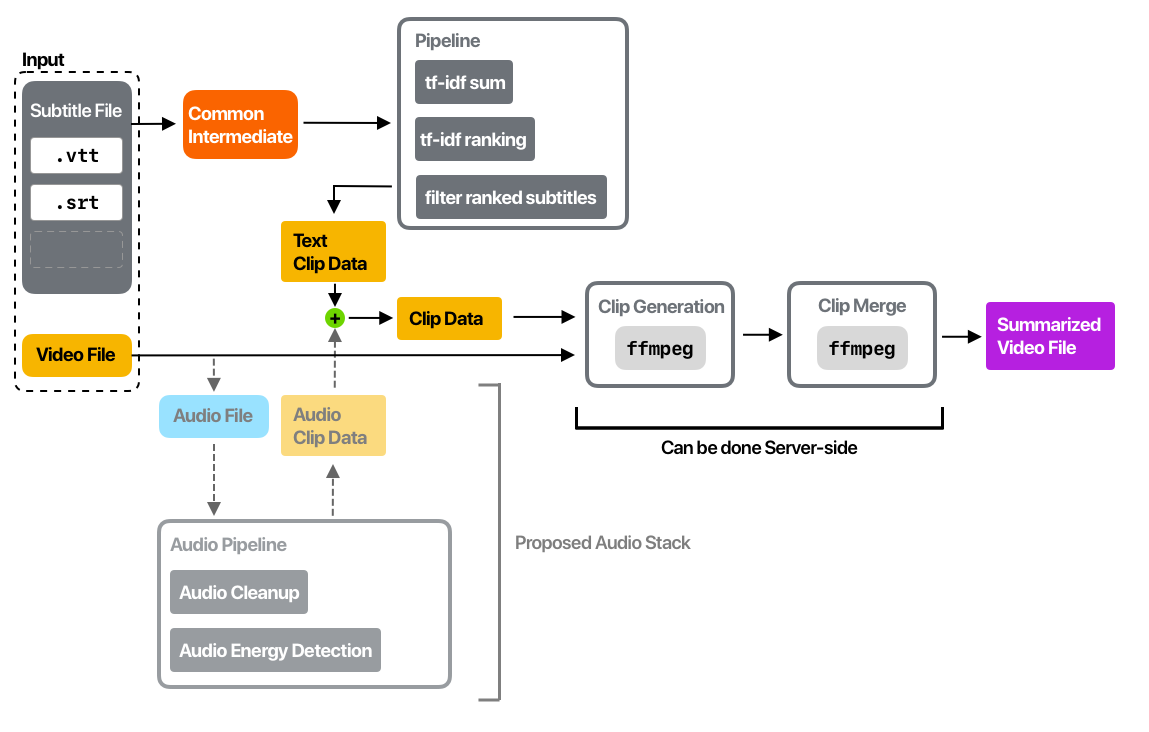
\includegraphics[width=0.8\textwidth, keepaspectratio=true]{Future}	
				\caption{Future Pipeline}
				\label{futurepipeline}
		\end{figure}

\begin{itemize}
			\item Completion of the implementation of the audio processing pipeline.
			\item Generation of subtitles for the final video.
			\item Determining the optimum value of the Flexibility Parameter, $F$ for the optimum summary length.
			\item Jarring cuts in video is to be minimized. This can be done by appropriately choosing the parameter \(N\) and implementing crossfade filters and other transitions in \verb|ffmpeg|.
		\end{itemize}
